\section{Experimental Validation}

To demonstrate the effectiveness of the model, I conducted tests by applying it to calibrate three different cameras: the Canon EOS D80, the iPhone X, and the Nikon D100. These cameras were chosen because they vary widely in terms of construction, image quality, and level of distortion. This diverse set of cameras provides a robust evaluation platform, allowing for an empirical assessment of the model's calibration performance, despite the small and statistically insignificant sample size.

To calibrate the camera, I first captured a picture of the calibration object of known dimensions using each of the cameras. In this case, the calibration object used consisted of 3 orthogonal planes with a checkerboard pattern imprinted onto each of the planes. The points at which the planes intersect was chosen to be the origin point of the world scene.

\begin{figure}[H]
    \centering
    \begin{subfigure}{0.5\textwidth}
        \centering
        \includegraphics[width=0.8\textwidth]{images/cal_object.png}
    \end{subfigure}%
    \begin{subfigure}{0.5\textwidth}
        \centering
        \includegraphics[width=0.9\textwidth]{images/cal_planes.png}
    \end{subfigure}
    \caption{Custom-made calibration object made using laser-cut MDF board. The checkerboard pattern was printed onto paper and glued onto the boards.}
\end{figure}

Then, I extracted the pixel coordinates of each of the points on the checkerboard and paired them to their corresponding real-world coordinates. This forms our dataset, which was then fed into a self-developed \emph{Python} program named \texttt{calicam}\footnote{See Appendix \ref{sec:source} for the source code of \texttt{calicam}.}. A subset of the dataset was earmarked to calibrate the model, used to solve for the projection matrix and extract intrinsic and extrinsic parameters. The remaining points were utilized for validation; the program reprojects these points and compares the estimated pixel coordinates of the projections to the ground truth provided in the dataset. By taking the average distances between the predicted points and their ground truths, we essentially calculate the reprojection error of the model, providing a quantitative measure of the accuracy of the predicted image coordinates compared to the actual observed values.

\begin{table}[H]
    \centering
    \resizebox{\columnwidth}{!}{
    \begin{tabular}{p{3cm}ccccccc}
        \toprule
                                                         &             & \multicolumn{2}{c}{\textbf{\small CANON D80}} & \multicolumn{2}{c}{\textbf{\small IPHONE X}} & \multicolumn{2}{c}{\textbf{\small NIKON D100}}                                                                               \\
        \cmidrule(lr){3-4}
        \cmidrule(lr){5-6}
        \cmidrule(lr){7-8}
                                                         &             & Spreaded Out                                  & Concentrated                                 & Spreaded Out                                   & Concentrated            & Spreaded Out            & Concentrated            \\
        \midrule
        \addlinespace
        \multirow{2}{*}{\footnotesize Focal Lengths}     & $f_x$       & $\qty{8404.1}{\pixel}$                        & $\qty{8305.9}{\pixel}$                       & $\qty{3281.5}{\pixel}$                         & $\qty{3125.7}{\pixel}$  & $\qty{8144.4}{\pixel}$  & $\qty{7716.4}{\pixel}$  \\
                                                         & $f_y$       & $\qty{8387.9}{\pixel}$                        & $\qty{8338.1}{\pixel}$                       & $\qty{3279.9}{\pixel}$                         & $\qty{3137.8}{\pixel}$  & $\qty{8142.6}{\pixel}$  & $\qty{7755.5}{\pixel}$  \\
        \addlinespace
        \multirow{2}{*}{\footnotesize Principal Point}   & $c_x$       & $\qty{3151.6}{\pixel}$                        & $\qty{3400.0}{\pixel}$                       & $\qty{2043.0}{\pixel}$                         & $\qty{2031.4}{\pixel}$  & $\qty{1541.8}{\pixel}$  & $\qty{1851.5}{\pixel}$  \\
                                                         & $c_y$       & $\qty{1972.8}{\pixel}$                        & $\qty{2075.8}{\pixel}$                       & $\qty{1453.1}{\pixel}$                         & $\qty{1467.4}{\pixel}$  & $\qty{1027.9}{\pixel}$  & $\qty{1205.4}{\pixel}$  \\
        \addlinespace
        \midrule
        \addlinespace
        \multirow{3}{*}{\footnotesize Tait-Bryan Angles} & $\alpha$    & $\qty{-81.86}{\degree}$                       & $\qty{-80.32}{\degree}$                      & $\qty{-60.21}{\degree}$                        & $\qty{-60.02}{\degree}$ & $\qty{-70.83}{\degree}$ & $\qty{-67.83}{\degree}$ \\
                                                         & $\beta$     & $\qty{44.27}{\degree}$                        & $\qty{46.00}{\degree}$                       & $\qty{38.72}{\degree}$                         & $\qty{38.28}{\degree}$  & $\qty{46.44}{\degree}$  & $\qty{48.43}{\degree}$  \\
                                                         & $\gamma$    & $\qty{4.97}{\degree}$                         & $\qty{5.98}{\degree}$                        & $\qty{21.64}{\degree}$                         & $\qty{21.81}{\degree}$  & $\qty{13.89}{\degree}$  & $\qty{16.04}{\degree}$  \\
        \addlinespace
        \multirow{3}{*}{\footnotesize Translation}       & $t_x$       & $\qty{494.8}{\mm}$                            & $\qty{492.9}{\mm}$                           & $\qty{329.0}{\mm}$                             & $\qty{317.4}{\mm}$      & $\qty{840.3}{\mm}$      & $\qty{801.1}{\mm}$      \\
                                                         & $t_y$       & $\qty{537.6}{\mm}$                            & $\qty{533.5}{\mm}$                           & $\qty{321.4}{\mm}$                             & $\qty{310.2}{\mm}$      & $\qty{766.0}{\mm}$      & $\qty{726.7}{\mm}$      \\
                                                         & $t_z$       & $\qty{128.3}{\mm}$                            & $\qty{130.5}{\mm}$                           & $\qty{208.6}{\mm}$                             & $\qty{202.1}{\mm}$      & $\qty{317.2}{\mm}$      & $\qty{306.8}{\mm}$      \\
        \addlinespace
        \midrule
        \addlinespace
        \multirow{2}{*}{\footnotesize Reproj. Errors}    & $\mu_{max}$ & $\qty{11.08}{\pixel}$                         & $\qty{17.21}{\pixel}$                        & $\qty{5.58}{\pixel}$                           & $\qty{19.48}{\pixel}$   & $\qty{11.70}{\pixel}$   & $\qty{14.13}{\pixel}$   \\
                                                         & $\mu_{avg}$ & $\qty{3.56}{\pixel}$                          & $\qty{7.36}{\pixel}$                         & $\qty{2.55}{\pixel}$                           & $\qty{4.86}{\pixel}$    & $\qty{2.81}{\pixel}$    & $\qty{5.04}{\pixel}$    \\
        \addlinespace
        \bottomrule
    \end{tabular}
}



    \caption{Intrinsic and Extrinsic Parameters calculated by \texttt{calicam}.}
\end{table}

The program is also capable of creating graphs by overlaying the image with the predicted image coordinates based on inputs. This feature enables users to visualize and compare the position of the predicted coordinates with the actual observed ones, providing a visual representation which can be used to empirically observe the model's performance.

\begin{figure}[H]
    \centering
    \begin{subfigure}{\textwidth}
        \centering
        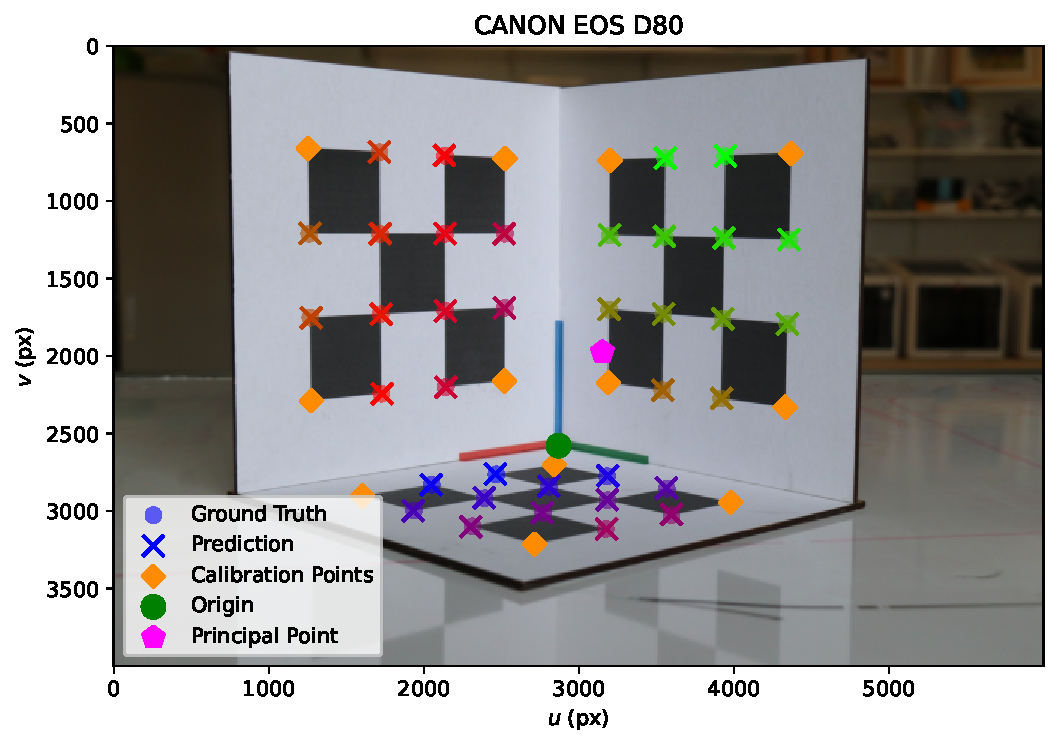
\includegraphics[width=0.75\textwidth]{assets/results/CANON EOS D80/graph.pdf}
        \caption{Canon EOS D80.}
    \end{subfigure}
    \begin{subfigure}{\textwidth}
        \centering
        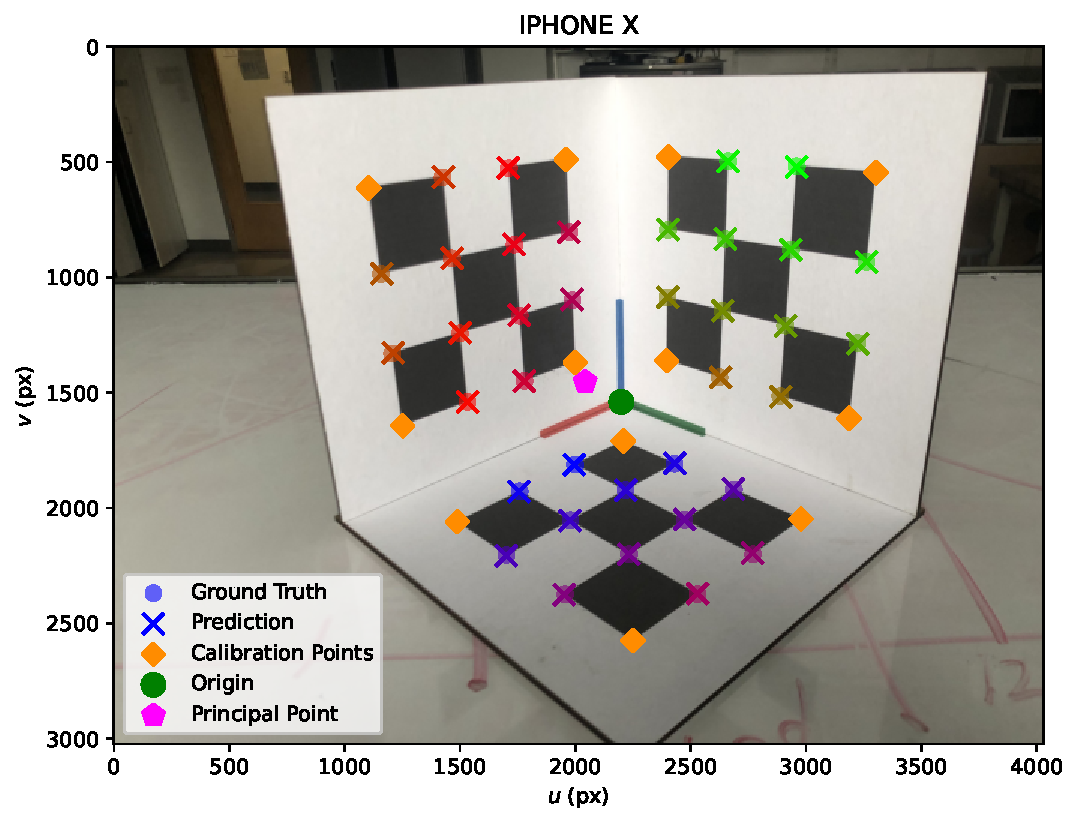
\includegraphics[width=0.75\textwidth]{assets/results/IPHONE X/graph.pdf}
        \caption{iPhone X.}
    \end{subfigure}
\end{figure}
\begin{figure}[H]
    \ContinuedFloat
    \centering
    \begin{subfigure}{\textwidth}
        \centering
        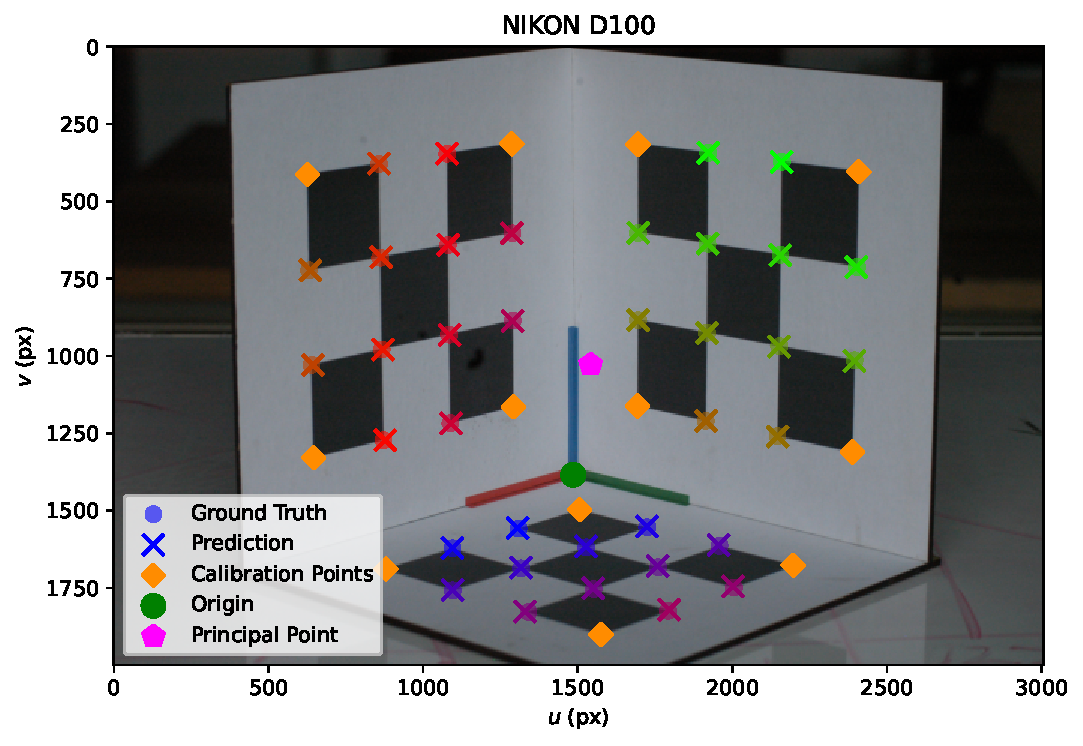
\includegraphics[width=0.75\textwidth]{assets/results/NIKON D100/graph.pdf}
        \caption{Nikon D100}
    \end{subfigure}
    \caption{Graphs generated by \texttt{calicam}.}
\end{figure}

\subsection{Validating Estimated Focal Length}
Given that specification of cameras are readily available online, we can actually further evaluate the accuracy of our model by calculating the focal lengths estimated by our model and comparing it to the manufacturer reported value. Assuming that the pixels are square, we estimate the focal lengths of our cameras to be the average of the horizontal and vertical focal lengths. Then, based on the manufacturer reported size of each individual pixel (known as the \emph{pixel pitch}), we can convert our estimated focal length from pixels to millimeters.

\begin{table}[H]
    \centering
    \resizebox{\columnwidth}{!}{
    \begin{tabular}{p{4.0cm}c@{\hskip 0.5cm}c@{\hskip 0.5cm}c}
        \toprule
                                      & \textbf{\small Calculated Focal Length}\tablefootnote{Pixel pitches retrieved from \url{digicamdb.com}.} & \textbf{\small Manufacturer Reported Focal Length} & \textbf{\small \% Error} \\
        \midrule
        \textbf{\small Canon EOS D80} & $(\qty{8496}{\pixel})(\qty{3.73e-3}{\milli\meter \per \pixel}) \approx \boxed{\qty{31.7}{\milli\meter}}$        & \qty{32}{\milli\meter}                & \qty{0.94}{\percent}     \\
        \textbf{\small IPhone X}      & $(\qty{3280}{\pixel})(\qty{1.22e-3}{\milli\meter \per \pixel}) \approx \boxed{\qty{4.00}{\milli\meter}}$        & \qty{4}{\milli\meter}                 & --                       \\
        \textbf{\small Nikon D100}    & $(\qty{8143}{\pixel})(\qty{7.82e-3}{\milli\meter \per \pixel}) \approx \boxed{\qty{63.7}{\milli\meter}}$        & \qty{55}{\milli\meter}                & \qty{15.6}{\percent}     \\
        \bottomrule
    \end{tabular}
}

    \caption{Comparison of Calculated vs. Manufacturer Reported Focal Length.}
\end{table}

Considering that the focal lengths reported by manufacturers are often only accurate to around $\pm \qty{1}{\milli\meter}$,\footcite{waynefAnswerAre2017} my results are very promising, with exception to the Nikon D100. However, this error is in fact a result of human error, as I forgot to turn off autofocus on the Nikon D100, and the zoom lens Nikon D100 altered the effective focal length.


